\section{Approach} \label{sec_approach}

\begin{figure}[t]
\centering
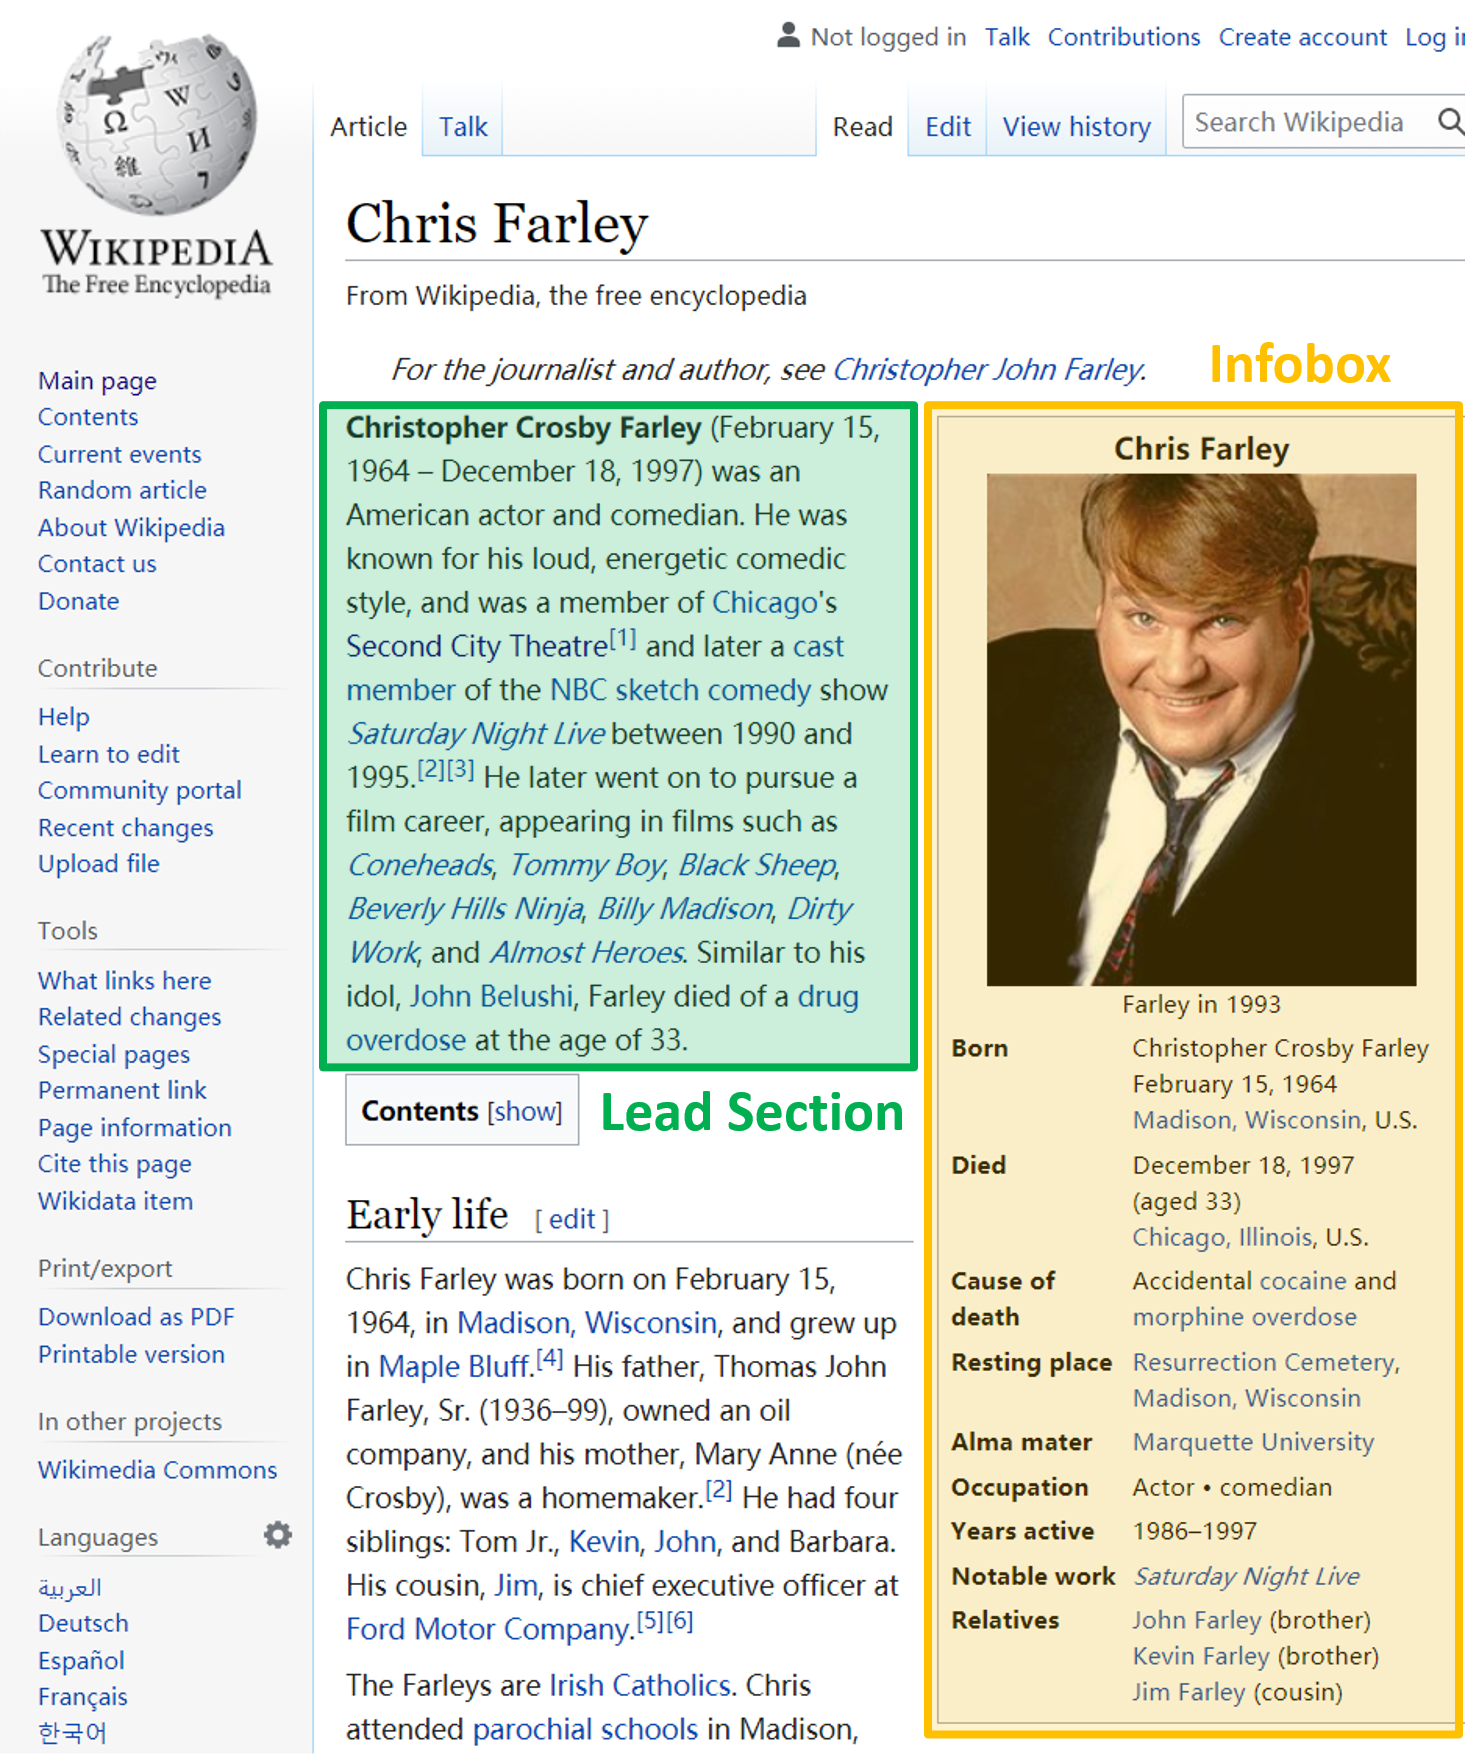
\includegraphics[width=1\columnwidth]{vis_example1}
\caption{The structure of a sample article with the lead section (green shading) and infobox (orange shading), followed by the start of the main content}
\label{vis_example1}
\end{figure}

\begin{figure}[t]
\centering
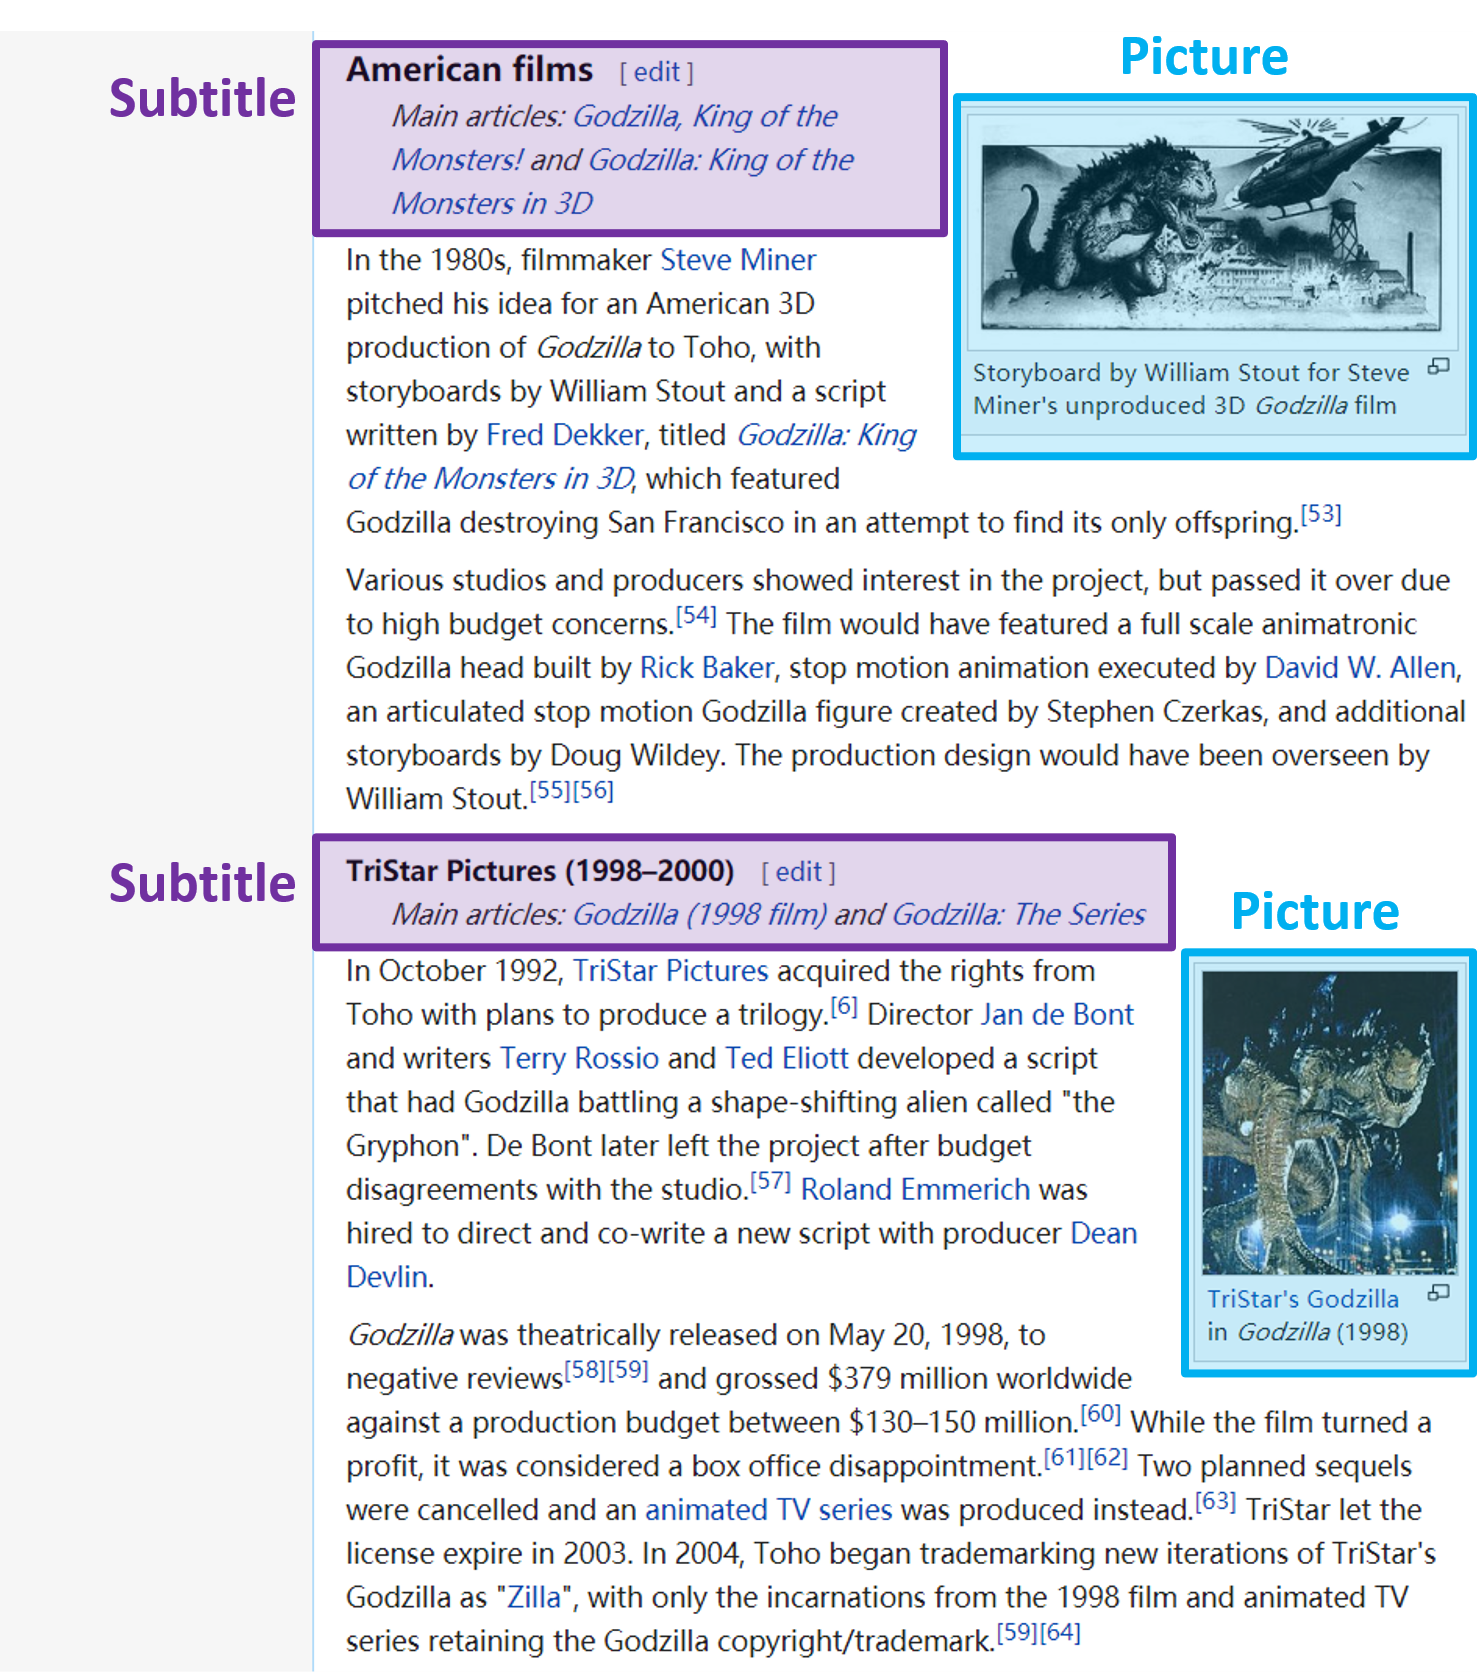
\includegraphics[width=1\columnwidth]{vis_example2}
\caption{The main content part of a sample article with subtitle (purple shading) and picture (blue shading)}
\label{vis_example2}
\end{figure}

This section introduces our approach to rank hyperlinks, which mainly takes two steps. We begin by obtaining the features of all the hyperlinks. Then, we feed these features into the Learning to Ranking algorithm.

\subsection{Learning to Rank}

Learning to Rank (LTR) is a supervised machine learning technique that aims to produce a ranking function $F$ with the set of feature vectors $\vec{x}$ to approximate the ground-truth rankings $y$. LTR is trained by optimizing the loss function $L(F(\vec{x_j}), y_j)$ for $1 \leq j \leq n$, which reflect the deviation of the predicted rankings from the ground-truth rankings. 

According to different realization of the loss function, L2R algorithms can be classified into 3 groups: pointwise, pairwise and listwise \cite{liu2011learning}. Listwise LTR algorithms like LambdaMart \cite{wu2010adapting} have shown competitive performance in many ranking tasks for their holistic utilization of the ranking list. Therefore, we choose LambdaMart as our ranking algorithm. 

\subsection{Visual Features}

Intuitively, how frequently a hyperlink gets clicked highly depends on its visual positions. Some regions are more exposed to the readers and can thus obtain more attention. It is reasonable to assume that users tend to click on links surrounded by pictures, subtitles and tables. In this paper, all the visual features we have proposed do not require rendering. Instead, we process the XML dump files and extract components with regular expressions. Here, we propose five visual features for hyperlink ranking: \emph{section position}, \emph{distance to the nearest picture}, \emph{distance to the nearest subtitle}, \emph{distance to nearest table} and \emph{within table}.

\subsubsection{Section Position}

In \cite{lamprecht2017structure}, the authors found that a large share of user clicks are from links in the lead section or in an infobox. We can exploit this finding as one of the features. Figure \ref{vis_example1} shows the beginning part of a sample article. In Figure \ref{vis_example1}, both the lead section and the infobox section have been highlighted. When browsing this web page, we tend to focus more on these two sections. For example, in the lead section, some hyperlinks like \emph{Coneheads} and \emph{Tommy Boy} usually get more clicks. Many hyperlinks in the rest sections remain unspotted until readers scroll down the web page. 

Therefore, hyperlinks in the first several sections are more likely to get frequently clicked. We propose a feature named \emph{section position} to represent which section the hyperlink is located in. The feature takes value of $x$ if the hyperlink is placed within the $x$th section.

\subsubsection{Picture}

Pictures are always eye-catching. When browsing web pages, readers tend to pay more attention to the pictures. Some links placed near to the picture are more likely to get clicked. For example in Figure \ref{vis_example2}, the hyperlink \emph{TriStar's Godzilla} is placed very near to a picture. We use \emph{distance to the nearest picture} as a feature to indicate whether the hyperlink is placed somewhere near to a picture.

\subsubsection{Subtitle}

Subtitles are highlighted in bold text with big fonts. The subtitle part is shown in Figure \ref{vis_example2}. When the readers start reading a paragraph under the subtitle, these hyperlinks near the subtitles are easier to be noticed. We assume that links near subtitles get more clicks, and propose \emph{distance to the nearest subtitle} as one of the visual features.
    
\subsubsection{Table}

Apart from pictures and titles, tables can also be attractive. In Figure \ref{vis_example3}, the hyperlink \emph{Apocalypto} is placed very near to the table, which is likely to get more clicks. We define the distance between the hyperlink and its nearest table as a feature called \emph{distance to the nearest table}.

We assume that whether a link is positioned within a table affects how frequently the hyperlink will get clicked. We propose \emph{within table} as another feature, which could help in predicting the click popularity of hyperlinks. If the link is placed within the table, the feature would take the value of 1, and 0 otherwise.

\begin{figure}[t]
\centering
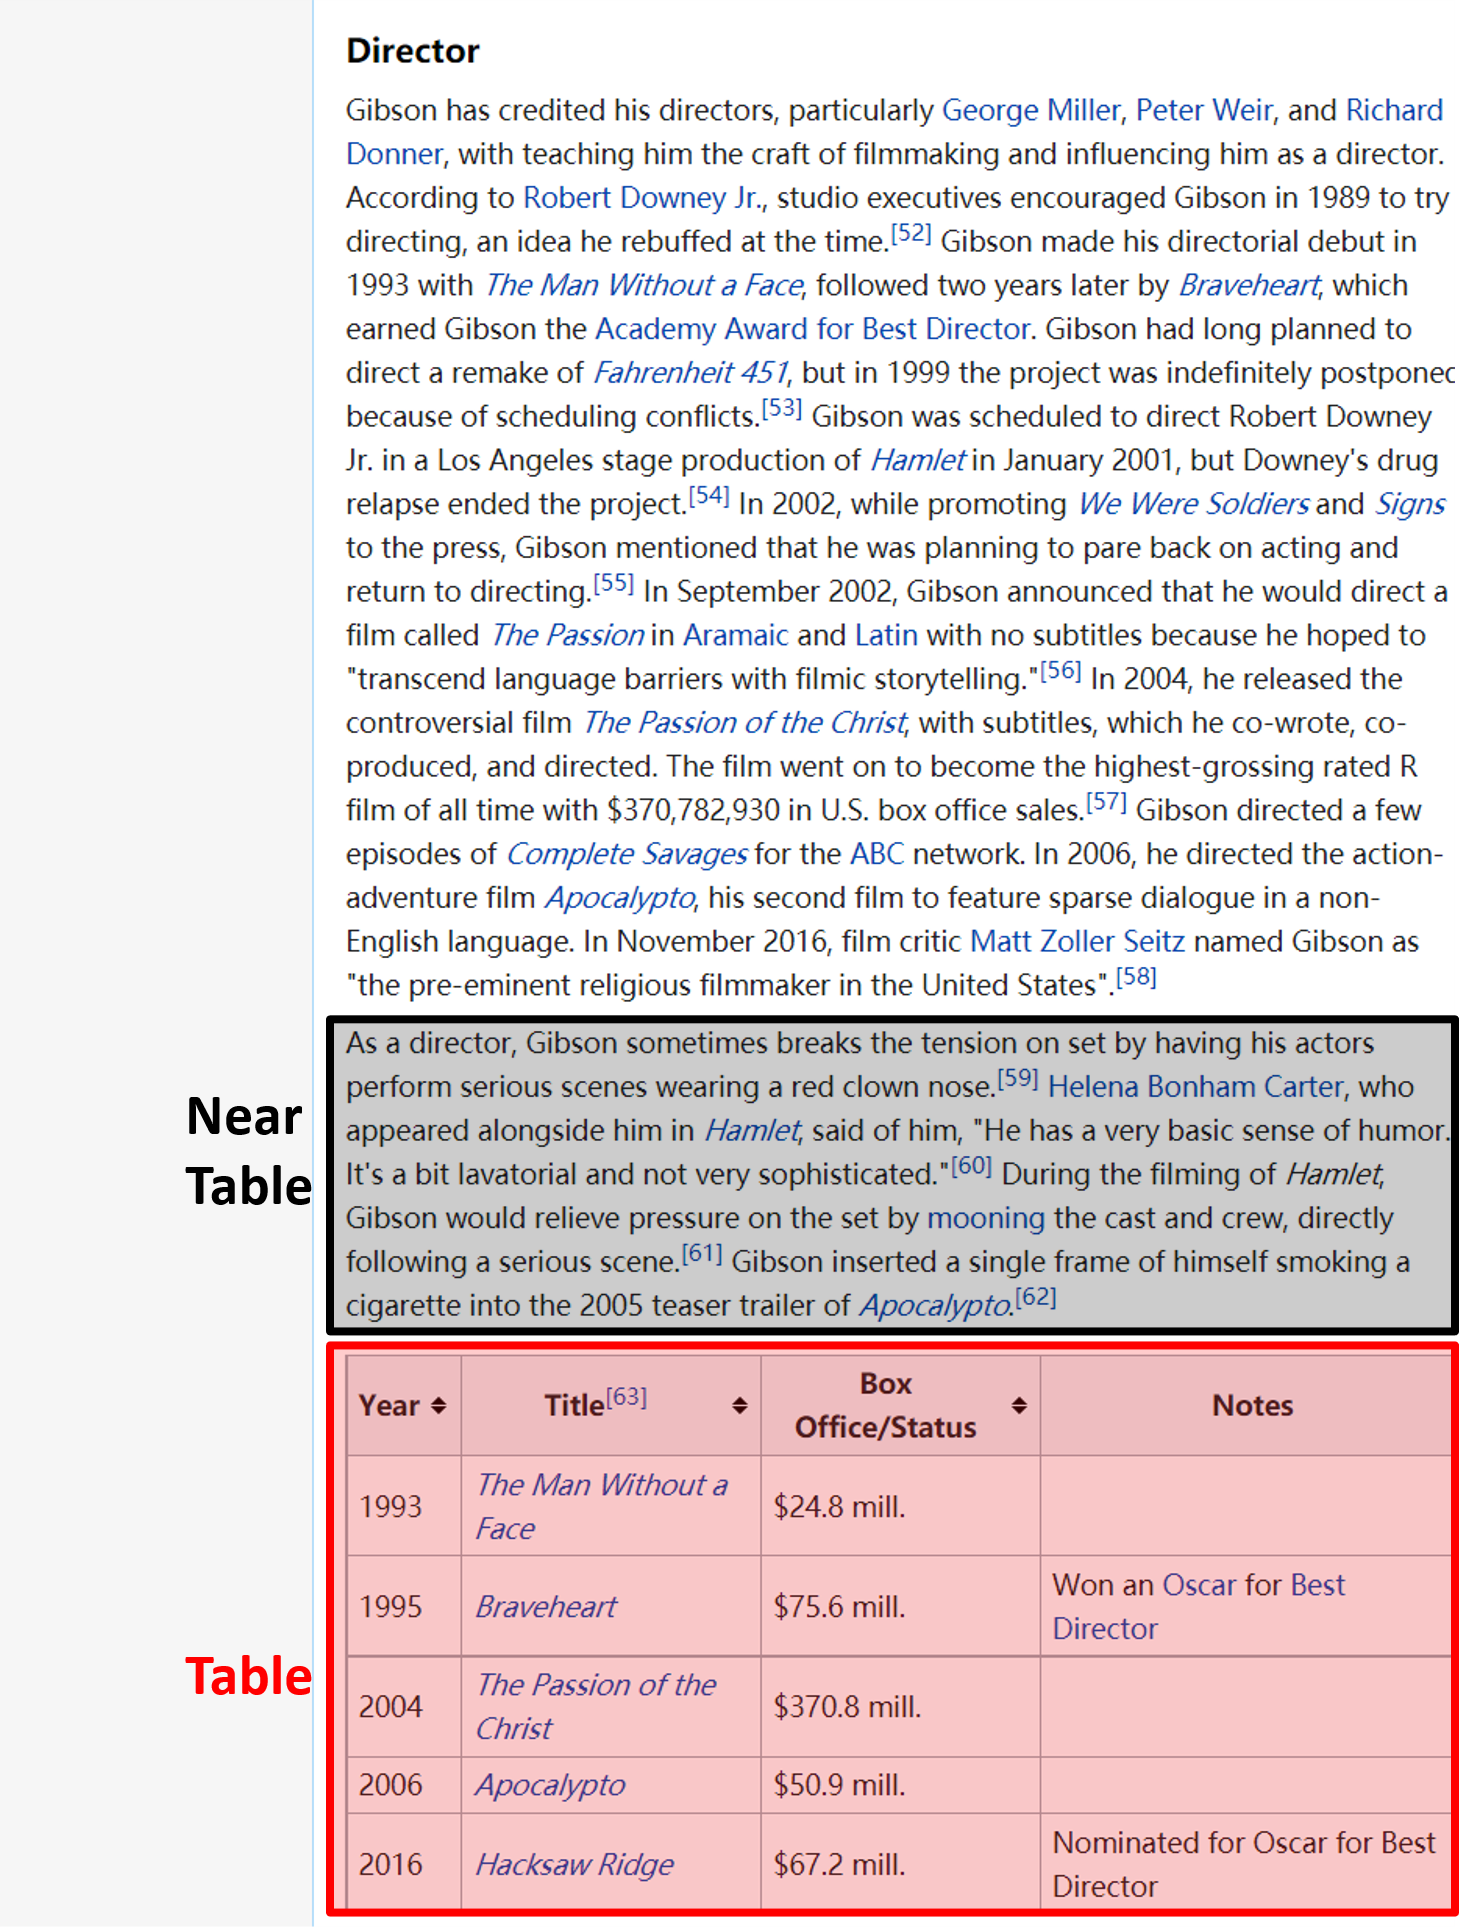
\includegraphics[width=1\columnwidth]{vis_example3}
\caption{The main content part of a sample article with near table section (black shading) and table (red shading)}
\label{vis_example3}
\end{figure}

\subsection{Textual Features}

The following textual features are used for ranking. We use $source$ and $dest$ to respectively denote the article the user is reading, and the article the hyperlinking is directing to.

\begin{itemize}

    \item[1.] \emph{Text Similarity}(\cite{thruesen2016link, dimitrov2017makes}): Cosine similarity of TF-IDF vectors between texts in $source$ and $dest$.

    \item[2.] \emph{Topic similarity(\cite{dimitrov2017makes})}: Cosine similarity of embedding vectors between Wikipedia categories assigned to $source$ and $dest$.

    \item[3.] \emph{Order}(\cite{thruesen2016link}): The $x$th hyperlink in the text.

    \item[4.] \emph{Number of links}(\cite{thruesen2016link}): The number of times the hyperlink appears in the article. 

    \item[5.] \emph{Position}(\cite{thruesen2016link}) and \emph{Log of Position}(\cite{thruesen2016link}): \emph{Position} and \emph{Log of Position} represents absolute and relative positions of hyperlinks in the article text.

    \item[6.] \emph{Topic similarity}(\cite{thruesen2016link}): The Jaccard coefficient of titles words in
    source and dest, which represents the similarity between two titles

\end{itemize}

\subsection{Graph-based Features}

All the articles together can be modeled as a graph. We introduce the following graph-based features.

\begin{itemize}

    \item[1.] \emph{In\_Degree}, \emph{Out\_Degree} and \emph{Degree} (\cite{dimitrov2017makes}): The in degree, out degree and degree of the article.

    \item[2.] \emph{K-Core Score}(\cite{dimitrov2017makes}): Score computed by K-Core measure

    \item[3.] \emph{PageRank Score}(\cite{thruesen2016link, dimitrov2017makes}): Score computed by Pagerank algorithm \cite{brin1998anatomy}.

    \item[4.] \emph{Symmetric link}(\cite{thruesen2016link}): The feature takes value from $\{0,1\}$, indicating whether or not the link is symmetric. A link $(source, dest)$ is considered symmetric if and only if the corresponding link $(dest, source)$ also exists. 

    \item[5.] \emph{Hub Score}(\cite{thruesen2016link}) and \emph{Authority Score}(\cite{thruesen2016link}): These two scores are calculated via HITS algorithm \cite{kleinberg1998authoritative}.

    \item[6.] \emph{Link Relatedness} (\cite{thruesen2016link}): The similarity between link sets of $source$ and $dest$, which contains their linked articles. Two metrics are computed by Jaccard coefficient and Dice's measure.

\end{itemize}

\subsection{Render Features}

The last feature groups is visual features from \cite{dimitrov2017makes}. To disambiguate between our visual feature, we name these previously proposed features as render features.

\begin{itemize}
    \item[1.] \emph{Lead or Body}: Whether the link is positioned in the lead section.

    \item[2.] \emph{Left or Right}: Whether the link is positioned in the left 10\% of the screen.

    \item[3.] \emph{Infobox}: Whether the link is placed within the Infobox.

    \item[4.] \emph{Navbox}: Whether the link is placed within the Navbox.

    \item[5.] \emph{screen x coord}: The x coordinate of the link.
    
    \item[6.] \emph{screen y coord}: The y coordinate of the link.
    
\end{itemize}